\documentclass[ucs,9pt]{beamer}

% Copyright 2004 by Till Tantau <tantau@users.sourceforge.net>.
%
% In principle, this file can be redistributed and/or modified under
% the terms of the GNU Public License, version 2.
%
% However, this file is supposed to be a template to be modified
% for your own needs. For this reason, if you use this file as a
% template and not specifically distribute it as part of a another
% package/program, I grant the extra permission to freely copy and
% modify this file as you see fit and even to delete this copyright
% notice.
%
% Modified by Tobias G. Pfeiffer <tobias.pfeiffer@math.fu-berlin.de>
% to show usage of some features specific to the FU Berlin template.

% remove this line and the "ucs" option to the documentclass when your editor is not utf8-capable
\usepackage[utf8x]{inputenc} % to make utf-8 input possible
\usepackage[english]{babel} % hyphenation etc., alternatively use 'german' as parameter

% Template for talks using the Corporate Design of the Freie Universitaet
%   Berlin, created following the guidelines on www.fu-berlin.de/cd by
%   Tobias G. Pfeiffer, <tobias.pfeiffer@math.fu-berlin.de>
% This file can be redistributed and/or modified in any way you like.
%   If you feel you have done significant improvements to this template,
%   please consider providing your modified version to
%   https://www.mi.fu-berlin.de/w/Mi/BeamerTemplateCorporateDesign

\usepackage{amsmath,dsfont,listings}

%%% FU logo
% small version for upper right corner of normal pages
\pgfdeclareimage[height=0.9cm]{university-logo}{FULogo_RGB}
\logo{\pgfuseimage{university-logo}}
% large version for upper right corner of title page
\pgfdeclareimage[height=1.085cm]{big-university-logo}{FULogo_RGB}
\newcommand{\titleimage}[1]{\pgfdeclareimage[height=2.92cm]{title-image}{#1}}
\titlegraphic{\pgfuseimage{title-image}}
%%% end FU logo

% NOTE: 1cm = 0.393 in = 28.346 pt;    1 pt = 1/72 in = 0.0352 cm
\setbeamersize{text margin right=3.5mm, text margin left=7.5mm}  % text margin

% colors to be used
\definecolor{text-grey}{rgb}{0.45, 0.45, 0.45} % grey text on white background
\definecolor{bg-grey}{rgb}{0.66, 0.65, 0.60} % grey background (for white text)
\definecolor{fu-blue}{RGB}{0, 51, 102} % blue text
\definecolor{fu-green}{RGB}{153, 204, 0} % green text
\definecolor{fu-red}{RGB}{204, 0, 0} % red text (used by \alert)

% switch off the sidebars
% TODO: loading \useoutertheme{sidebar} (which is maybe wanted) also inserts
%   a sidebar on title page (unwanted), also indents the page title (unwanted?),
%   and duplicates the navigation symbols (unwanted)
\setbeamersize{sidebar width left=0cm, sidebar width right=0mm}
\setbeamertemplate{sidebar right}{}
\setbeamertemplate{sidebar left}{}
%    XOR
% \useoutertheme{sidebar}

% frame title
% is truncated before logo and splits on two lines
% if neccessary (or manually using \\)
\setbeamertemplate{frametitle}{%
    \vskip-30pt \color{text-grey}\large%
    \begin{minipage}[b][23pt]{80.5mm}%
    \flushleft\insertframetitle%
    \end{minipage}%
}

%%% title page
% TODO: get rid of the navigation symbols on the title page.
%   actually, \frame[plain] *should* remove them...
\setbeamertemplate{title page}{
% upper right: FU logo
\vskip2pt\hfill\pgfuseimage{big-university-logo} \\
\vskip6pt\hskip3pt
% title image of the presentation
\begin{minipage}{11.6cm}
\hspace{-1mm}\inserttitlegraphic
\end{minipage}

% set the title and the author
\vskip14pt
\parbox[top][1.35cm][c]{11cm}{\color{text-grey}\inserttitle \\ \small \insertsubtitle}
\vskip11pt
\parbox[top][1.35cm][c]{11cm}{\small \insertauthor \\ \insertinstitute \\[3mm] \insertdate}
}
%%% end title page

%%% colors
\usecolortheme{lily}
\setbeamercolor*{normal text}{fg=black,bg=white}
\setbeamercolor*{alerted text}{fg=fu-red}
\setbeamercolor*{example text}{fg=fu-green}
\setbeamercolor*{structure}{fg=fu-blue}

\setbeamercolor*{block title}{fg=white,bg=black!50}
\setbeamercolor*{block title alerted}{fg=white,bg=black!50}
\setbeamercolor*{block title example}{fg=white,bg=black!50}

\setbeamercolor*{block body}{bg=black!10}
\setbeamercolor*{block body alerted}{bg=black!10}
\setbeamercolor*{block body example}{bg=black!10}

\setbeamercolor{bibliography entry author}{fg=fu-blue}
% TODO: this doesn't work at all:
\setbeamercolor{bibliography entry journal}{fg=text-grey}

\setbeamercolor{item}{fg=fu-blue}
\setbeamercolor{navigation symbols}{fg=text-grey,bg=bg-grey}
%%% end colors

%%% headline
\setbeamertemplate{headline}{
\vskip4pt\hfill\insertlogo\hspace{3.5mm} % logo on the right

\vskip6pt\color{fu-blue}\rule{\textwidth}{0.4pt} % horizontal line
}
%%% end headline

%%% footline
\newcommand{\footlinetext}{\insertshortinstitute, \insertshorttitle, \insertshortdate}
\setbeamertemplate{footline}{
\vskip5pt\color{fu-blue}\rule{\textwidth}{0.4pt}\\ % horizontal line
\vskip2pt
\makebox[123mm]{\hspace{7.5mm}
\color{fu-blue}\footlinetext
\hfill \raisebox{-1pt}{\usebeamertemplate***{navigation symbols}}
\hfill \insertframenumber}
\vskip4pt
}
%%% end footline

%%% settings for listings package
\lstset{extendedchars=true, showstringspaces=false, basicstyle=\footnotesize\sffamily, tabsize=2, breaklines=true, breakindent=10pt, frame=l, columns=fullflexible}
\lstset{language=Java} % this sets the syntax highlighting
\lstset{mathescape=true} % this switches on $...$ substitution in code
% enables UTF-8 in source code:
\lstset{literate={ä}{{\"a}}1 {ö}{{\"o}}1 {ü}{{\"u}}1 {Ä}{{\"A}}1 {Ö}{{\"O}}1 {Ü}{{\"U}}1 {ß}{\ss}1}
%%% end listings % THIS is the line that includes the FU template!

\usepackage{arev,t1enc} % looks nicer than the standard sans-serif font
% if you experience problems, comment out the line above and change
% the documentclass option "9pt" to "10pt"

\usepackage{graphicx}

% image to be shown on the title page (without file extension, should be pdf or png)
\titleimage{fu_500}

\title[Jail++] % (optional, use only with long paper titles)
{\textbf{Jail++} \newline Rail to JBC Compiler in C++}

\subtitle
{Pr\"asentiert von Jail Constructions Ltd. (auch bekannt als C++ Gruppe)}

\author[Jail Constructions Ltd.] % (optional, use only with lots of authors)
{Jail Constructions Ltd.}
% - Give the names in the same order as the appear in the paper.

\institute[FU Berlin] % (optional, but mostly needed)
{Freie Universität Berlin}
% - Keep it simple, no one is interested in your street address.

\date[SWP Compilerbau 2014] % (optional, should be abbreviation of conference name)
{Softwareprojekt \"Ubersetzerbau, 2014}
% - Either use conference name or its abbreviation.
% - Not really informative to the audience, more for people (including
% yourself) who are reading the slides online

\subject{Sofwareprojekt \"Ubersetzerbau}
% This is only inserted into the PDF information catalog. Can be left
% out.

% you can redefine the text shown in the footline. use a combination of
% \insertshortauthor, \insertshortinstitute, \insertshorttitle, \insertshortdate, ...
\renewcommand{\footlinetext}{\insertshortinstitute, \insertshorttitle, \insertshortdate}


\begin{document}

\begin{frame}[plain]
  \titlepage
\end{frame}

\subsection{Übersicht}

\begin{frame}{Übersicht}
  \begin{itemize}
  	\pause
  	\item Organisation
  	\pause
  	\item Frontend
  	\pause
  	\item Backend
  	\pause
  	\item Editor
  	\pause
  	\item Fazit
  \end{itemize}
\end{frame}
\subsection{Organisation}

\begin{frame}{Organisation}

\begin{figure}
  \begin{center}
    \leavevmode
      \includegraphics[width = .75\textwidth]{organisation}
    \caption{Scrum Master und Product Owner}
  \end{center}
\end{figure}

\end{frame}

\pagebreak

\begin{frame}{Organisation}

	\pause
	\"Ubersicht:
	\pause
	\begin{itemize}
		\item Anforderungen, Ziele und Prozesse
		\pause
		\item Team-Aufteilung 
		\pause
		\item Aufgetretene Probleme und gefundene L\"osungen
		\pause
		\item Verwendete Tools
		\pause
		\item Vorstellung der Compiler Pipeline
	\end{itemize}

\end{frame}

\pagebreak

\begin{frame}{Organisation: Anforderungen, Ziele und Prozesse}

	\pause
	\begin{itemize}
		\item Bau eines Compilers f\"ur Rail in C++ zu Java Bytecode (selbstgew\"ahltes Target)
		\pause
		\item Rail ist eine zweidimensionale, esoterische Programmiersprache 
		\pause
		\item Der komplette Sprachumfang soll umgesetzt werden
		\pause
		\item Dieses \"ubergeordnete Ziel wurde unterteilt in 3 Meilensteine:
		\pause
		\begin{itemize}
			\item \textbf{\textcolor{fu-blue}{MS 1}}  Grundlegendes Parsen der Schienen, Strings und Konsolenausgabe
			\pause
			\item \textbf{\textcolor{fu-blue}{MS 2}}  Arithmetische Operationen, Verzweigungen (if-else) und Variablen
			\pause
			\item \textbf{\textcolor{fu-blue}{MS 3}}  Kompletter Sprachumfang: Funktionsaufrufe, Rekursion, Schleifen 
		\end{itemize}
	\end{itemize}

\end{frame}
	
\begin{frame}{Organisation: Anforderungen, Ziele und Prozesse}

	\pause
	\begin{itemize}
		\item Zus\"atzliche Anforderungen:
		\pause
		\begin{itemize}
			\item \textbf{\textcolor{fu-blue}{Cross-Kompatibilit\"at}} Erstellung eines austauschbaren Dateiformats f\"ur den AST
			\pause
			\item \textbf{\textcolor{fu-blue}{Cross-Testing}} Testen der Compiler der zwei Gruppen mit Ast-Dateien der jeweils anderen Gruppe
			\pause
			\item \textbf{\textcolor{fu-blue}{IDE}} Eine f\"ur Rail spezialisierte Entwicklungsumgebung soll umgesetzt werden
			\pause
		\end{itemize}
		\item Prozess ist Scrum-\"ahnlich:
		\pause
		\begin{itemize}
			\item Meilensteine (Sprints)
			\pause
			\item Stand-up Meetings
			\pause
			\item Retrospektiven (am Ende der Meilensteine)
			\pause
			\item Rollen wie Scrum Master und Product Owner
		\end{itemize}
	\end{itemize}

\end{frame}

\pagebreak


\begin{frame}{Verwendete Tools}

	\pause
	\begin{itemize}
		\item Teamspeak
		\pause
		\item Jabber
		\pause
		\item Mail 
		\pause
		\item Github als Codebase
		\pause
		\item Keine festgelegte Entwicklungsumgebung f\"ur C++
		\pause
		\item Jenkins und Gradle f\"ur Continuous Integration
		\pause
		\item Qt f\"ur die Entwicklung des Editors
		\pause
		\item Doxygen f\"ur automatisierte Dokumentationserzeugung
	\end{itemize}


\end{frame}


\begin{frame}{Organisation: Team-Aufteilung}

\begin{figure}
  \begin{center}
    \leavevmode
      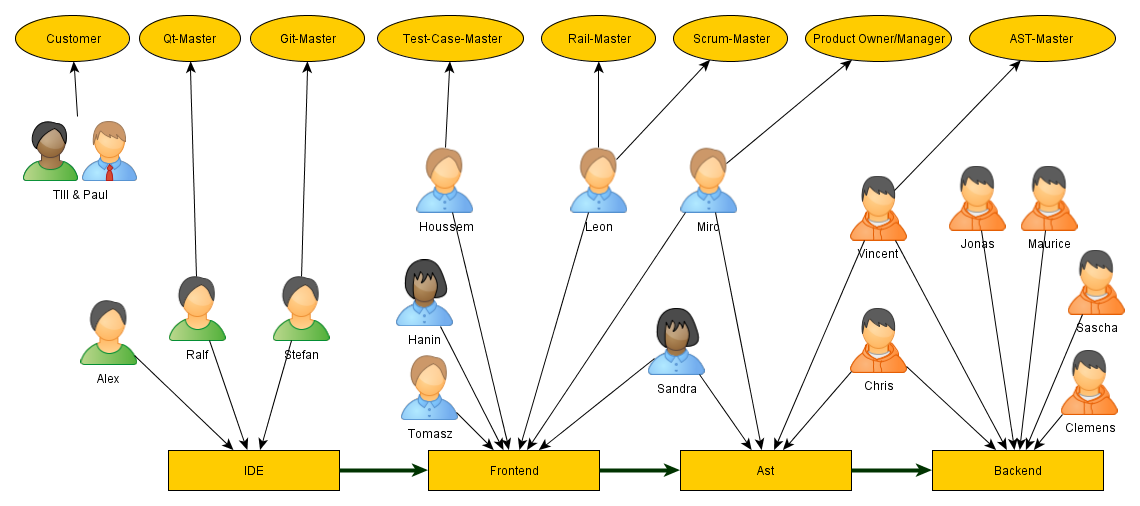
\includegraphics[width = \textwidth]{organigram}
    \caption{Organigramm}
  \end{center}
\end{figure}

\end{frame}

\pagebreak

\begin{frame}{Organisation: Aufgetretene Probleme und gefundene L\"osungen}
	
	\pause
	\begin{itemize}
		\item Probleme in MS 1:
		\pause
		\begin{itemize}
			\item Kommunikation (kein einheitliches Tool, seltene Treffen)
			\pause
			\item Unklare bzw. ungleiche Arbeitsaufteilung
			\pause
		\end{itemize}
		\item Verbessert durch:
		\pause
		\begin{itemize}
			\item Einf\"uhrung von Daily-Scrums $\rightarrow$ 3 Treffen pro Subteam w\"ochentlich (Voice-Chat)
			\pause
			\item Scrum-Master und Product Owner sind bei allen Treffen anwesend $\rightarrow$ besserer Gesamt\"uberblick
			\pause
			\item Nutzung der Github-Issues zur Verbesserung und Klarstellung der Aufgabenverteilung
			\pause
			\item Jabber f\"ur spontane Kommunikation
		\end{itemize}
	\end{itemize}
	
\end{frame}

\begin{frame}{Vorstellung der Compiler Pipeline}

\begin{figure}
  \begin{center}
    \leavevmode
      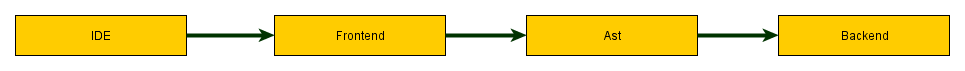
\includegraphics[width = \textwidth]{pipeline}
    \caption{Compiler Pipeline und Subteams}
  \end{center}
\end{figure}

\end{frame}

\subsection{Frontend}

\begin{frame}{Frontend}

	\begin{figure}
	  \begin{center}
	    \leavevmode
	      \includegraphics[width = .75\textwidth]{frontend}
	    \caption{Team Frontend}
	  \end{center}
	\end{figure}

\end{frame}

\begin{frame}{Frontend}

	\pause
	\"Ubersicht:
	\pause
	\begin{itemize}
		\item Softwaretechnik
		\pause
		\item Technische Aspekte
	\end{itemize}

\end{frame}

\pagepreak


\begin{frame}{Frontend: Softwaretechnik}
	
	\pause
	\begin{itemize}
		\item Sechs Teammitglieder
		\pause
		\item Austausch mit Haskell-Gruppe: Design der AST-Datei
		\pause
		\item Kommunikation wie im Organisationsteil erw\"ahnt
		\pause
		\item T\"atigkeitsfelder:
		\pause
		\begin{itemize}
			\item Lexer
			\pause
			\item Parser
			\pause
			\item AST Serialisierung/Deserialisierung
			\pause
			\item Rail-Testcases
			\pause
			\item Testing-Framework
		\end{itemize}
	\end{itemize}
	
\end{frame}

\pagebreak
\begin{frame}{Frontend: Softwaretechnik}

	\begin{itemize}
		\item Wichtige Erkenntnisse
		\pause
		\begin{itemize}
			\item Gelernte Theorie l\"asst sich nur begrenzt anwenden
			\pause
			\item Praktische Umst\"ande verlangen individuelle L\"osungen
			\pause
			\item Ein guter Entwurf spart enormen Aufwand
		\end{itemize}
	\end{itemize}
	
\pagebreak

\end{frame}

\begin{frame}{Frontend: Softwaretechnik}

\begin{figure}
  \begin{center}
    \leavevmode
      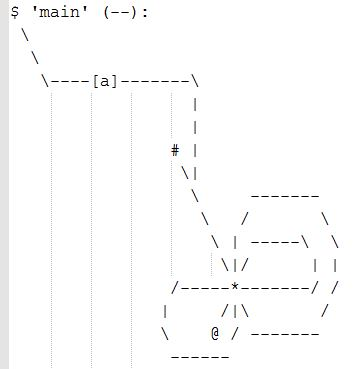
\includegraphics[width = .5\textwidth]{rail}
    \caption{Grammatik hierf\"ur?}
  \end{center}
\end{figure}

	
\end{frame}

\begin{frame}{Frontend: Technisches}

\begin{figure}
  \begin{center}
    \leavevmode
      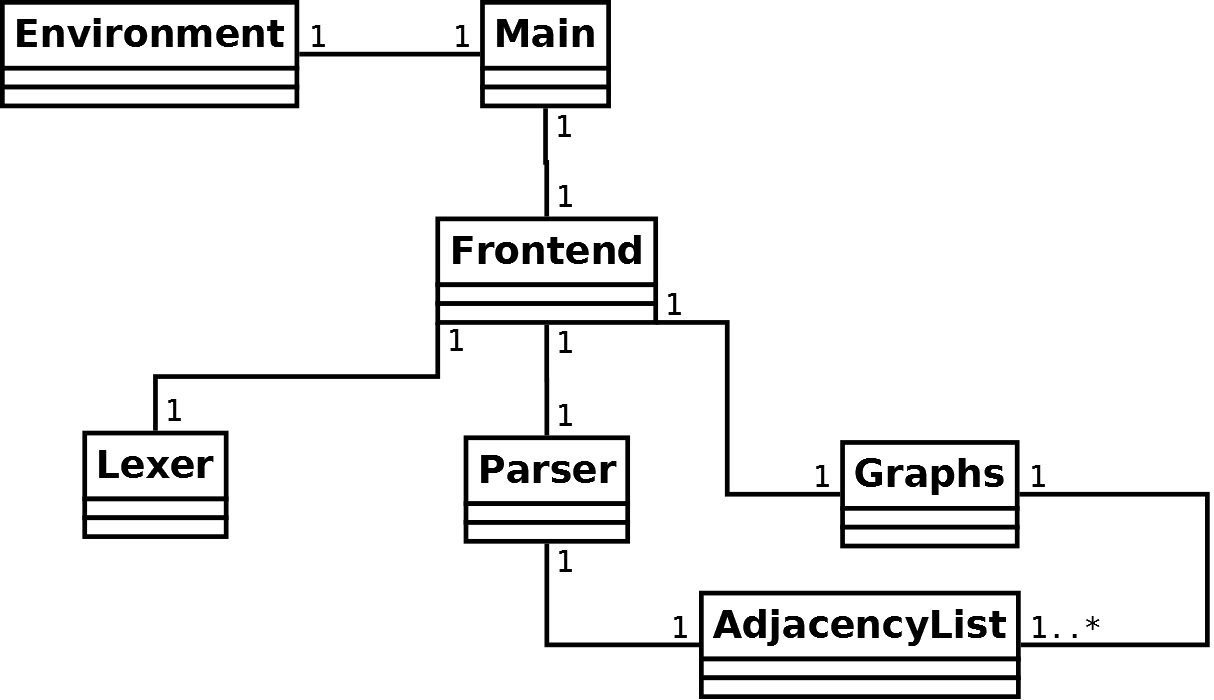
\includegraphics[width = \textwidth]{frontenduml}
    \caption{Klassendiagramm Frontend}
  \end{center}
\end{figure}

\end{frame}

\begin{frame}{Frontend: Technisches}

Die Hauptarbeit geschieht im Parser:
\pause
\begin{itemize}
	\item Durchlaufen der Funktion anhand der Schienen
	\pause
	\item Aufbau einer Graph-Struktur durch den Parser
	\pause
	\item F\"ur jeden gesehenen Rail-Befehl wird gespeichert:
	\pause
	\begin{itemize}
		\item Position
		\pause
		\item Richtung
		\pause
		\item Befehl
		\pause
	\end{itemize}
	\item Verkn\"upfen dieser Informationen mit dem Knoten verhindert mehrfaches Parsen
	\pause
	\item Verzweigungen durch rekursive Selbstaufrufe
	\pause
	\item F\"ur anonyme Funktionen (Lambda) werden neue Funktionsnamen generiert und die Funktionen geparst
	\pause
	\item Erzeugt f\"ur jede Rail-Funktion einen Graphen
\end{itemize}

\end{frame}

\subsection{Backend}

\begin{frame}[fragile]{Backend}
	\begin{figure}
	  \begin{center}
	    \leavevmode
	      \includegraphics[width = .75\textwidth]{backend}
	    \caption{Team Backend}
	  \end{center}
	\end{figure}
\end{frame}

\begin{frame}[fragile]{JVM Bytecode und Classfile}
% NB. listings is quite powerful, but not well suited to be used with beamer
%  consider using semiverbatim or the like, see below
\begin{lstlisting}[language=Java]
public class HelloWorld{
	  public static void main(String[] args){
	    System.out.println("Hello World");
	  }	
}
\end{lstlisting}
\end{frame}

\begin{frame}[fragile]{Classfile Beispiel}
\begin{center}
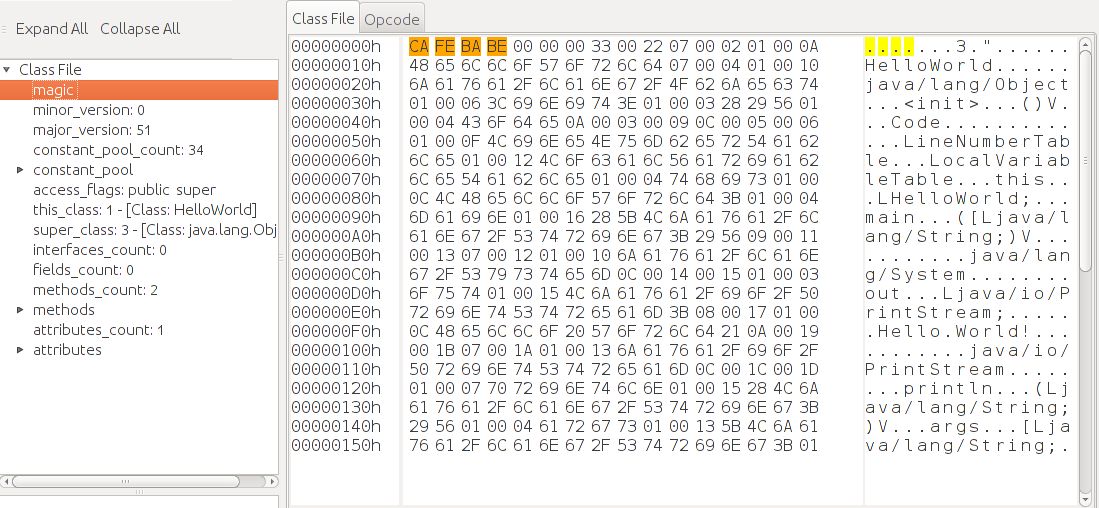
\includegraphics[width=\textwidth]{class1}
\end{center}
\end{frame}

\begin{frame}[fragile]{Classfile Beispiel II}
\begin{center}
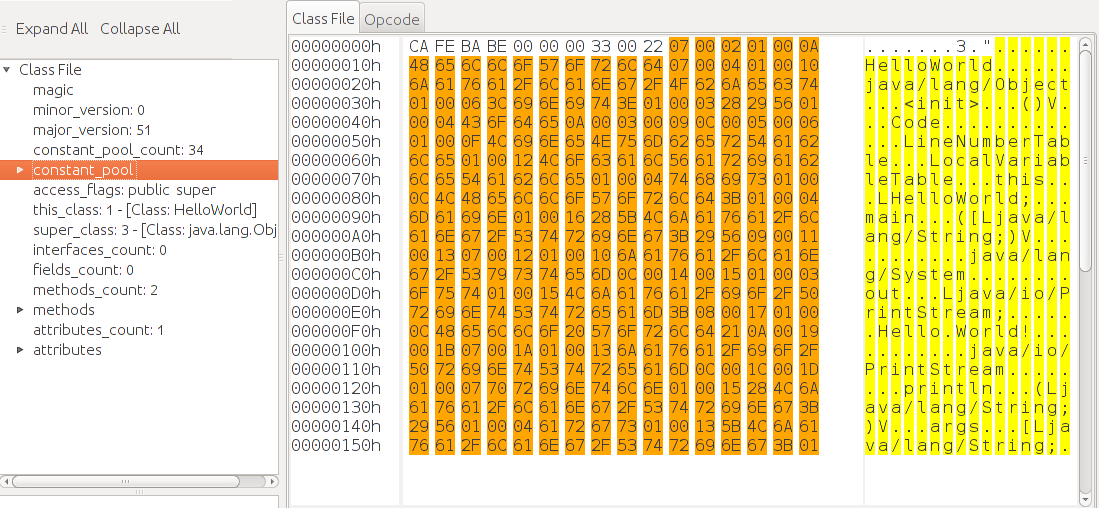
\includegraphics[width=\textwidth]{class2}
\end{center}
\end{frame}

\begin{frame}[fragile]{Classfile Beispiel III}
\begin{center}
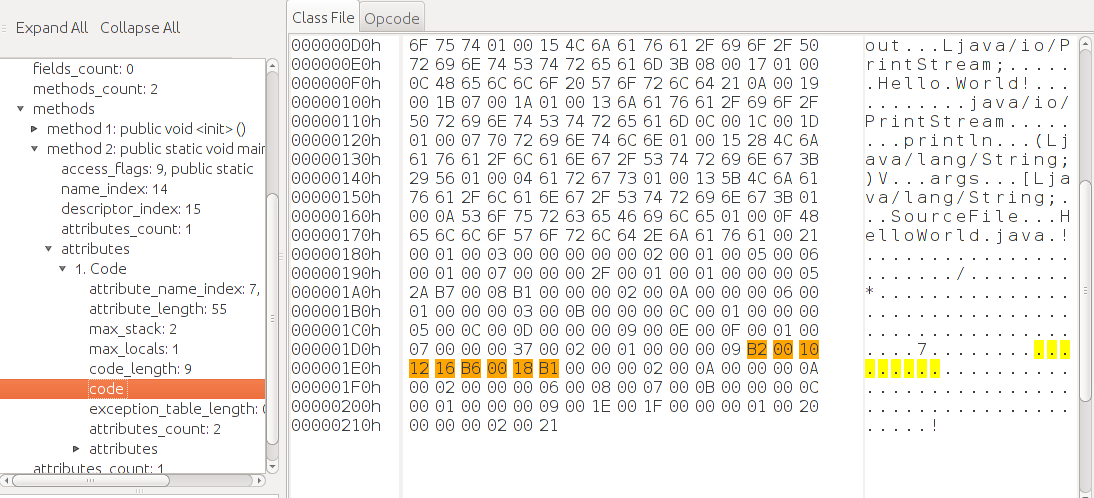
\includegraphics[width=\textwidth]{class3}
\end{center}
\end{frame}

\begin{frame}[fragile]{Classfile Beispiel IV}
\begin{center}
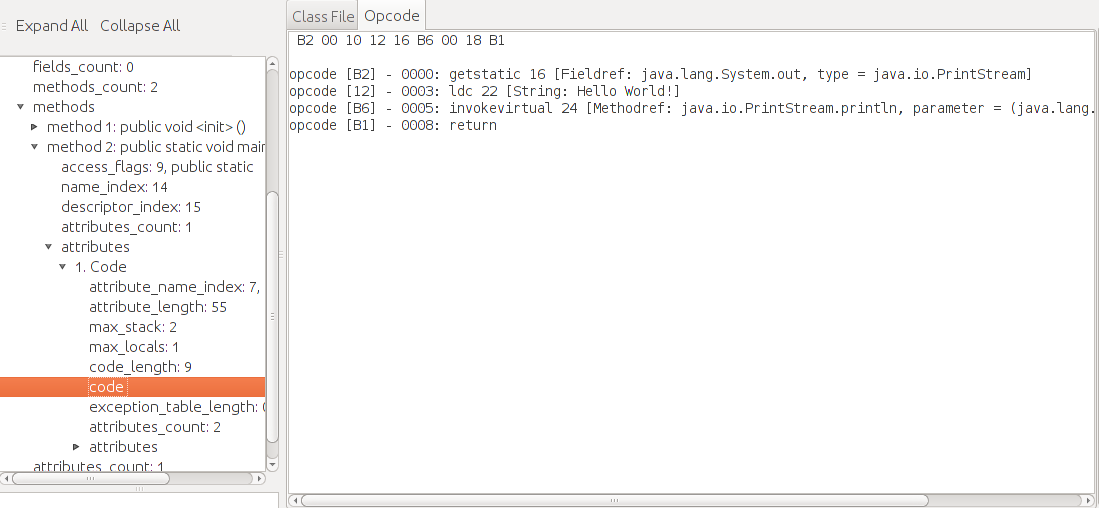
\includegraphics[width=\textwidth]{class4}
\end{center}
\end{frame}

\begin{frame}[fragile]{Backend Klassendiagramm Übersicht}
\begin{center}
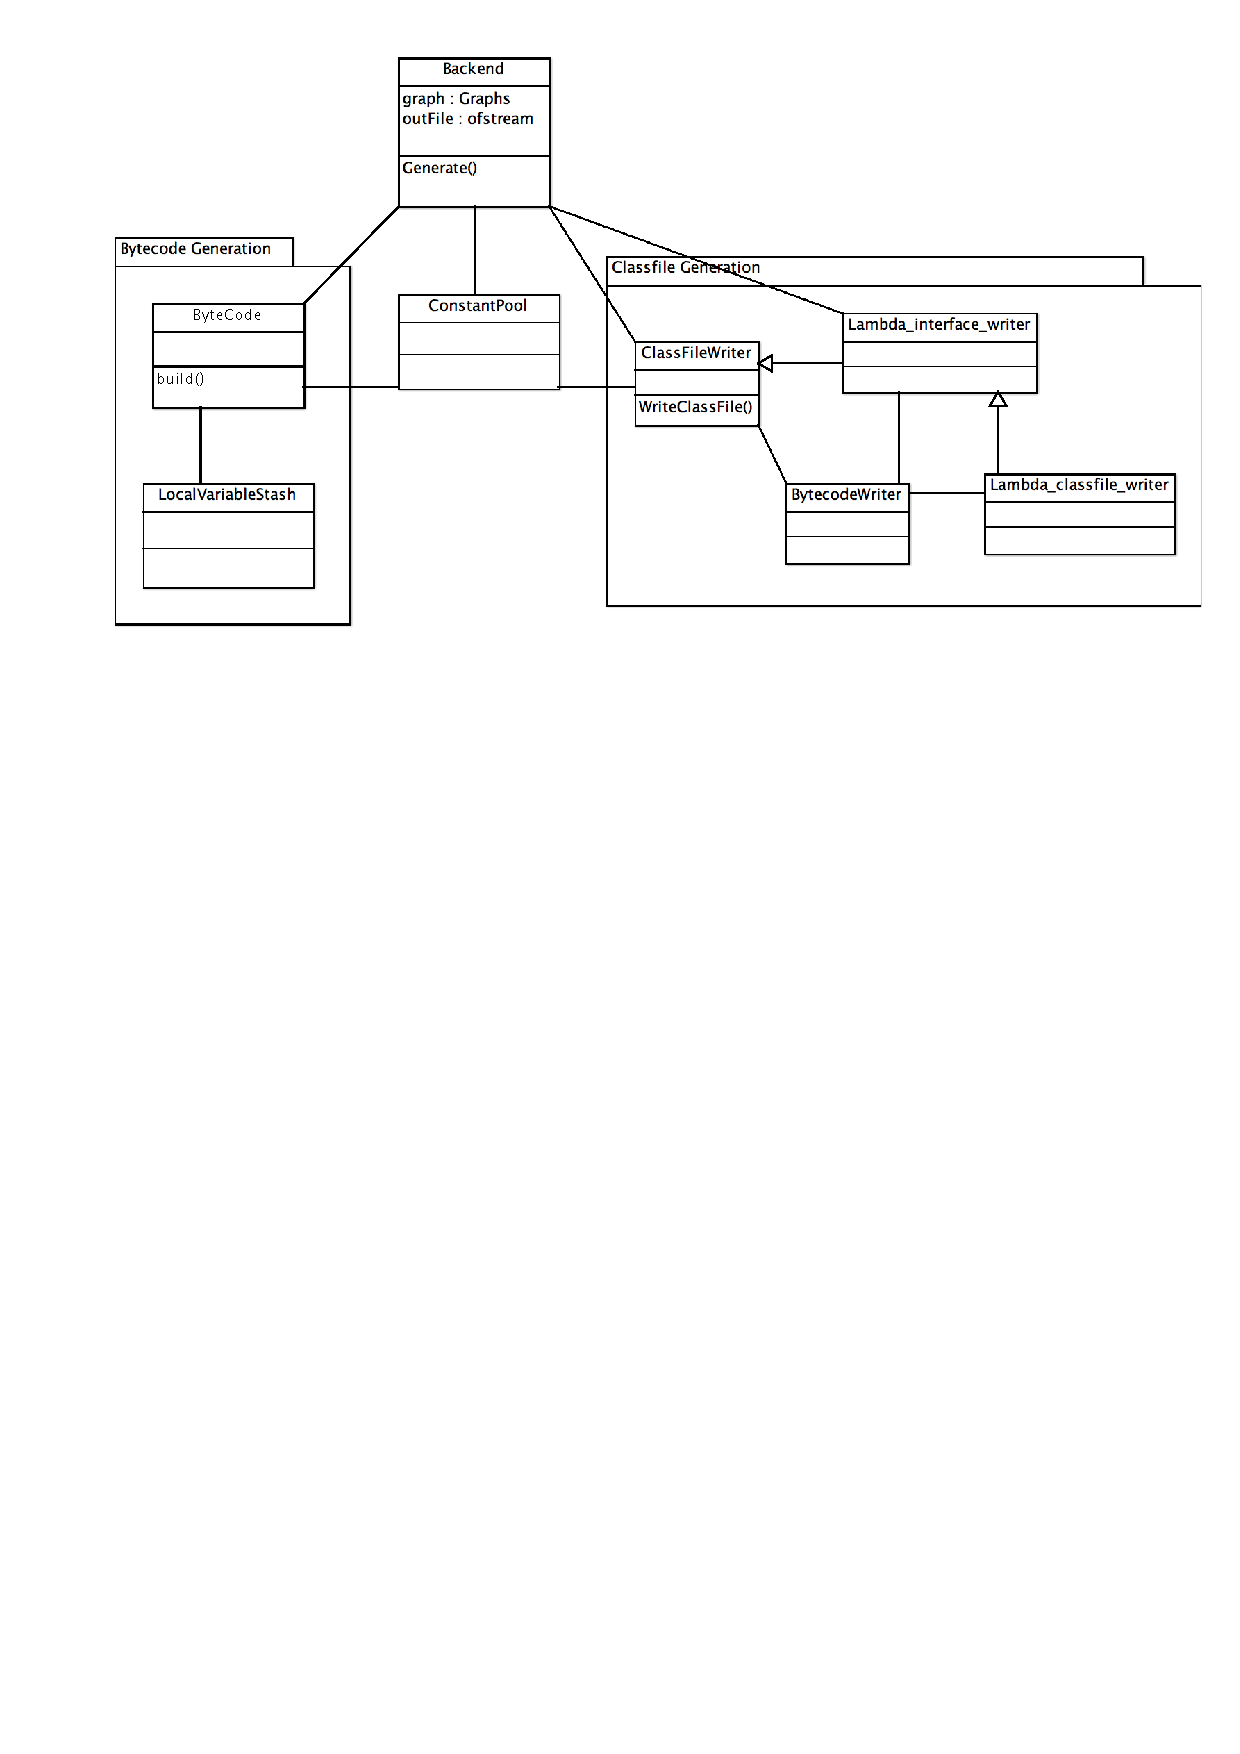
\includegraphics[width=\textwidth]{class}
\end{center}
\end{frame}

\begin{frame}[fragile]{Backend Sequenzdiagramm Übersicht}
\begin{figure}[htp]
\begin{center}
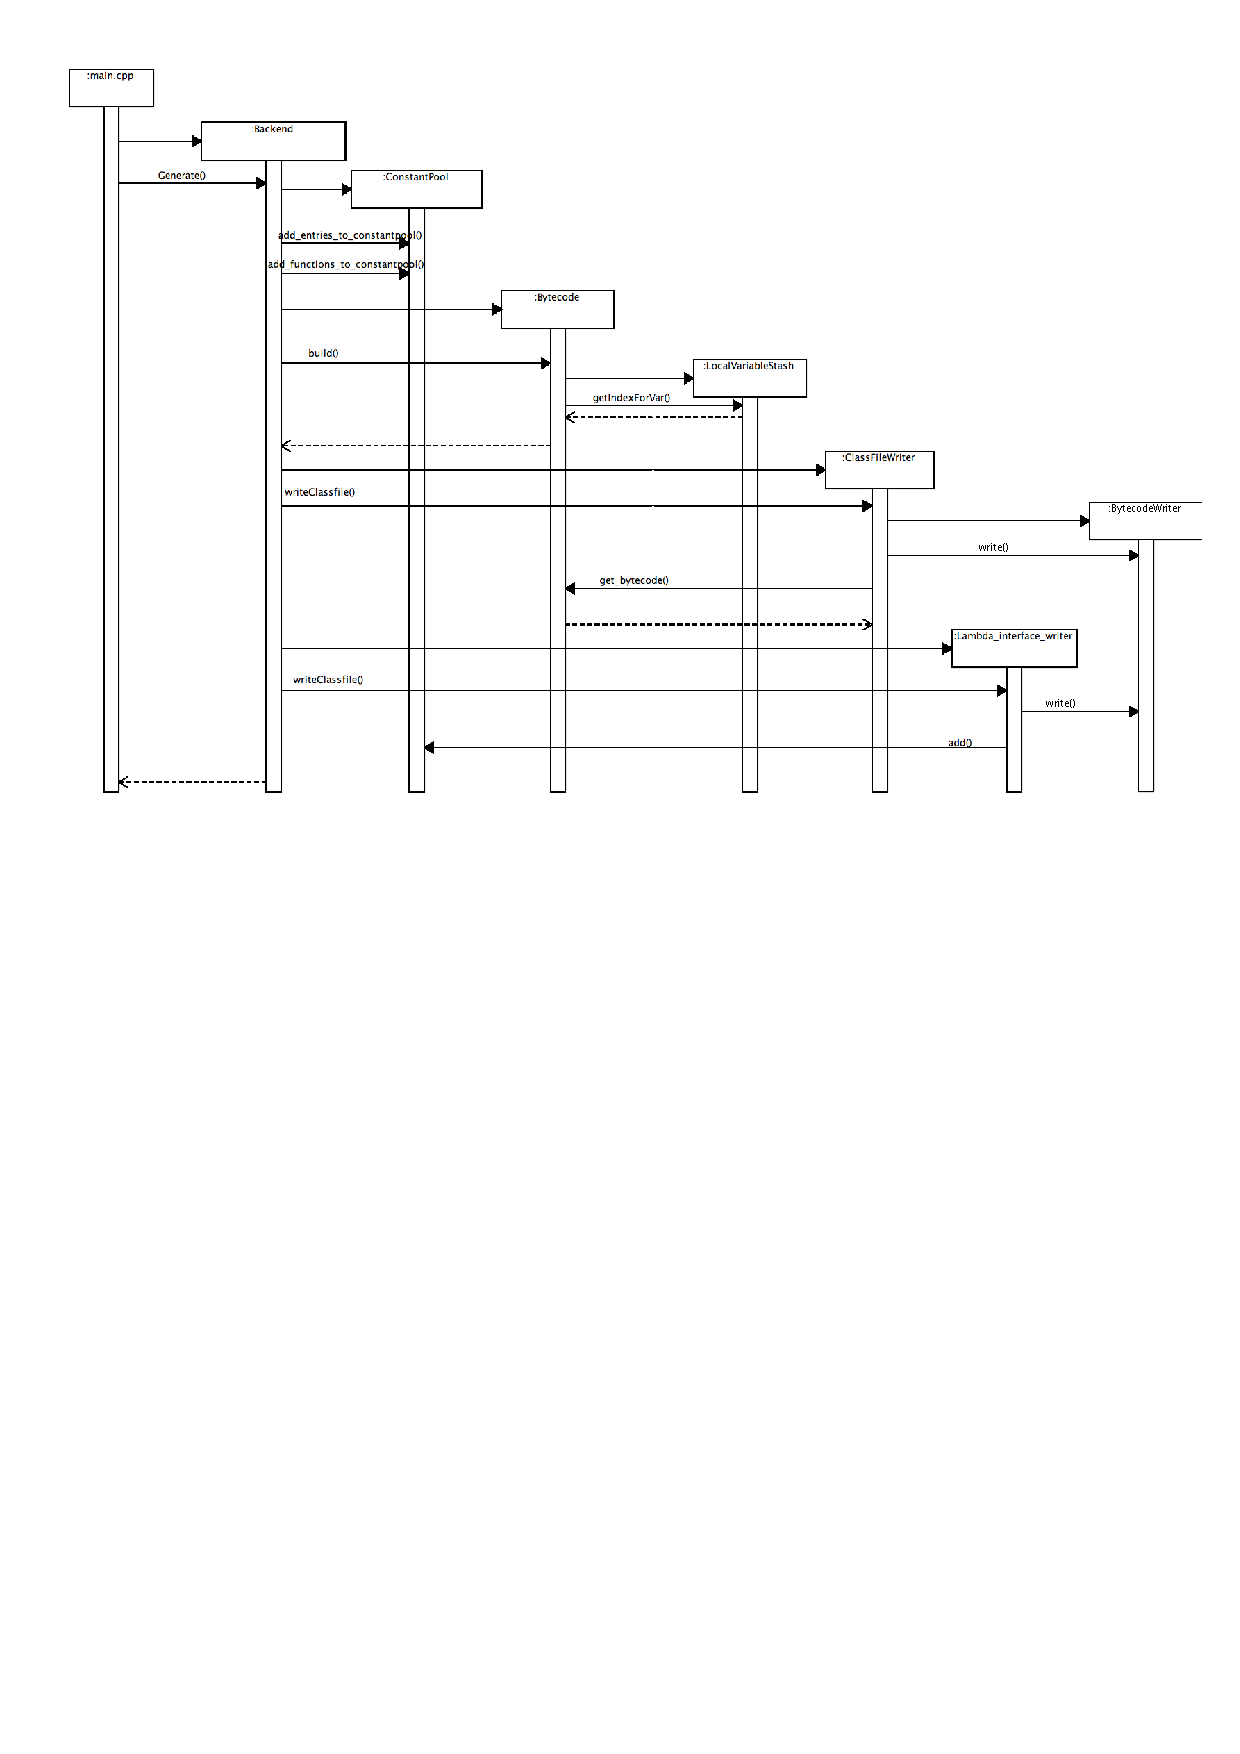
\includegraphics[width=\textwidth]{Sequenz}
\end{center}
\end{figure}
\end{frame}

\begin{frame}[fragile]{Backend Sequenzdiagramm Erster Teil}
\begin{figure}[htp]
\begin{center}
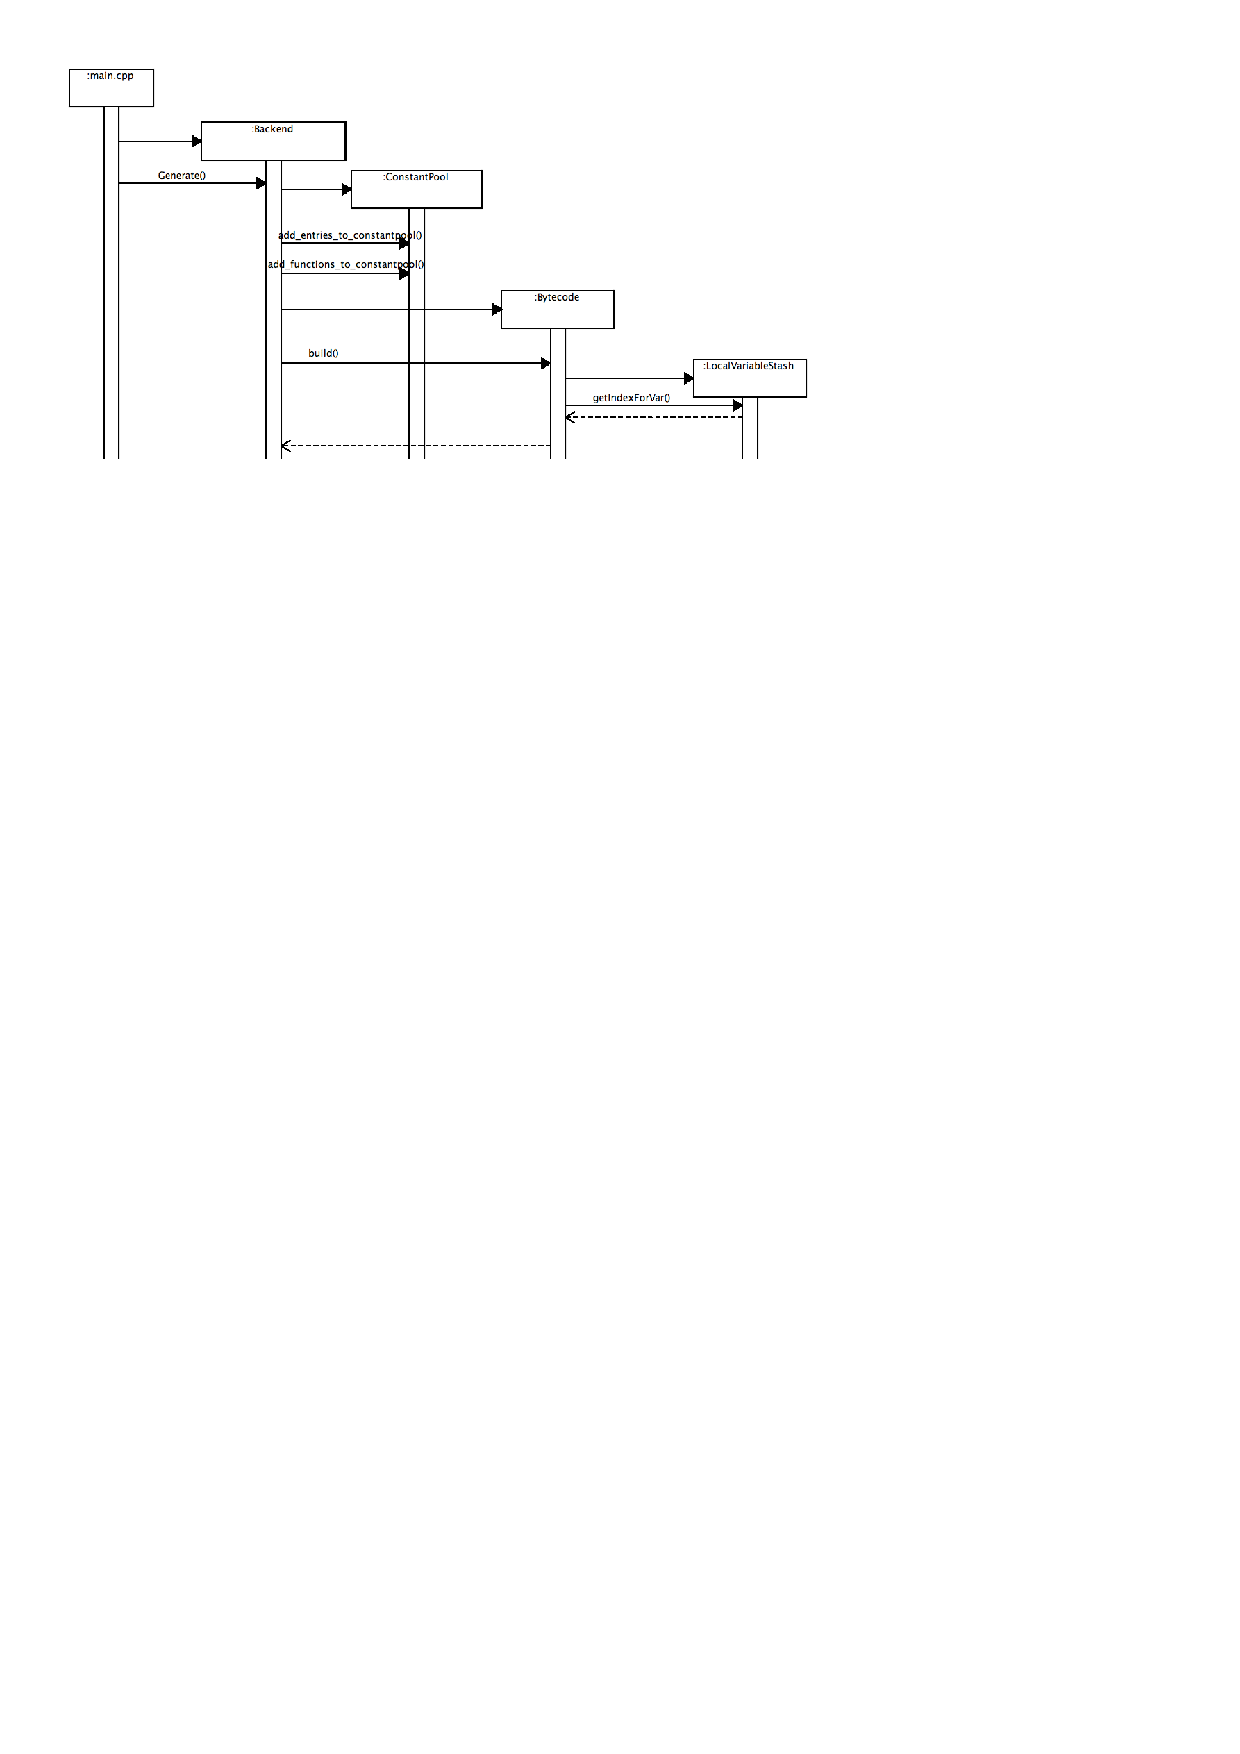
\includegraphics[width=\textwidth]{oben}
\end{center}
\end{figure}
\end{frame}

\begin{frame}[fragile]{Backend Sequenzdiagramm Übersicht}
\begin{figure}[htp]
\begin{center}
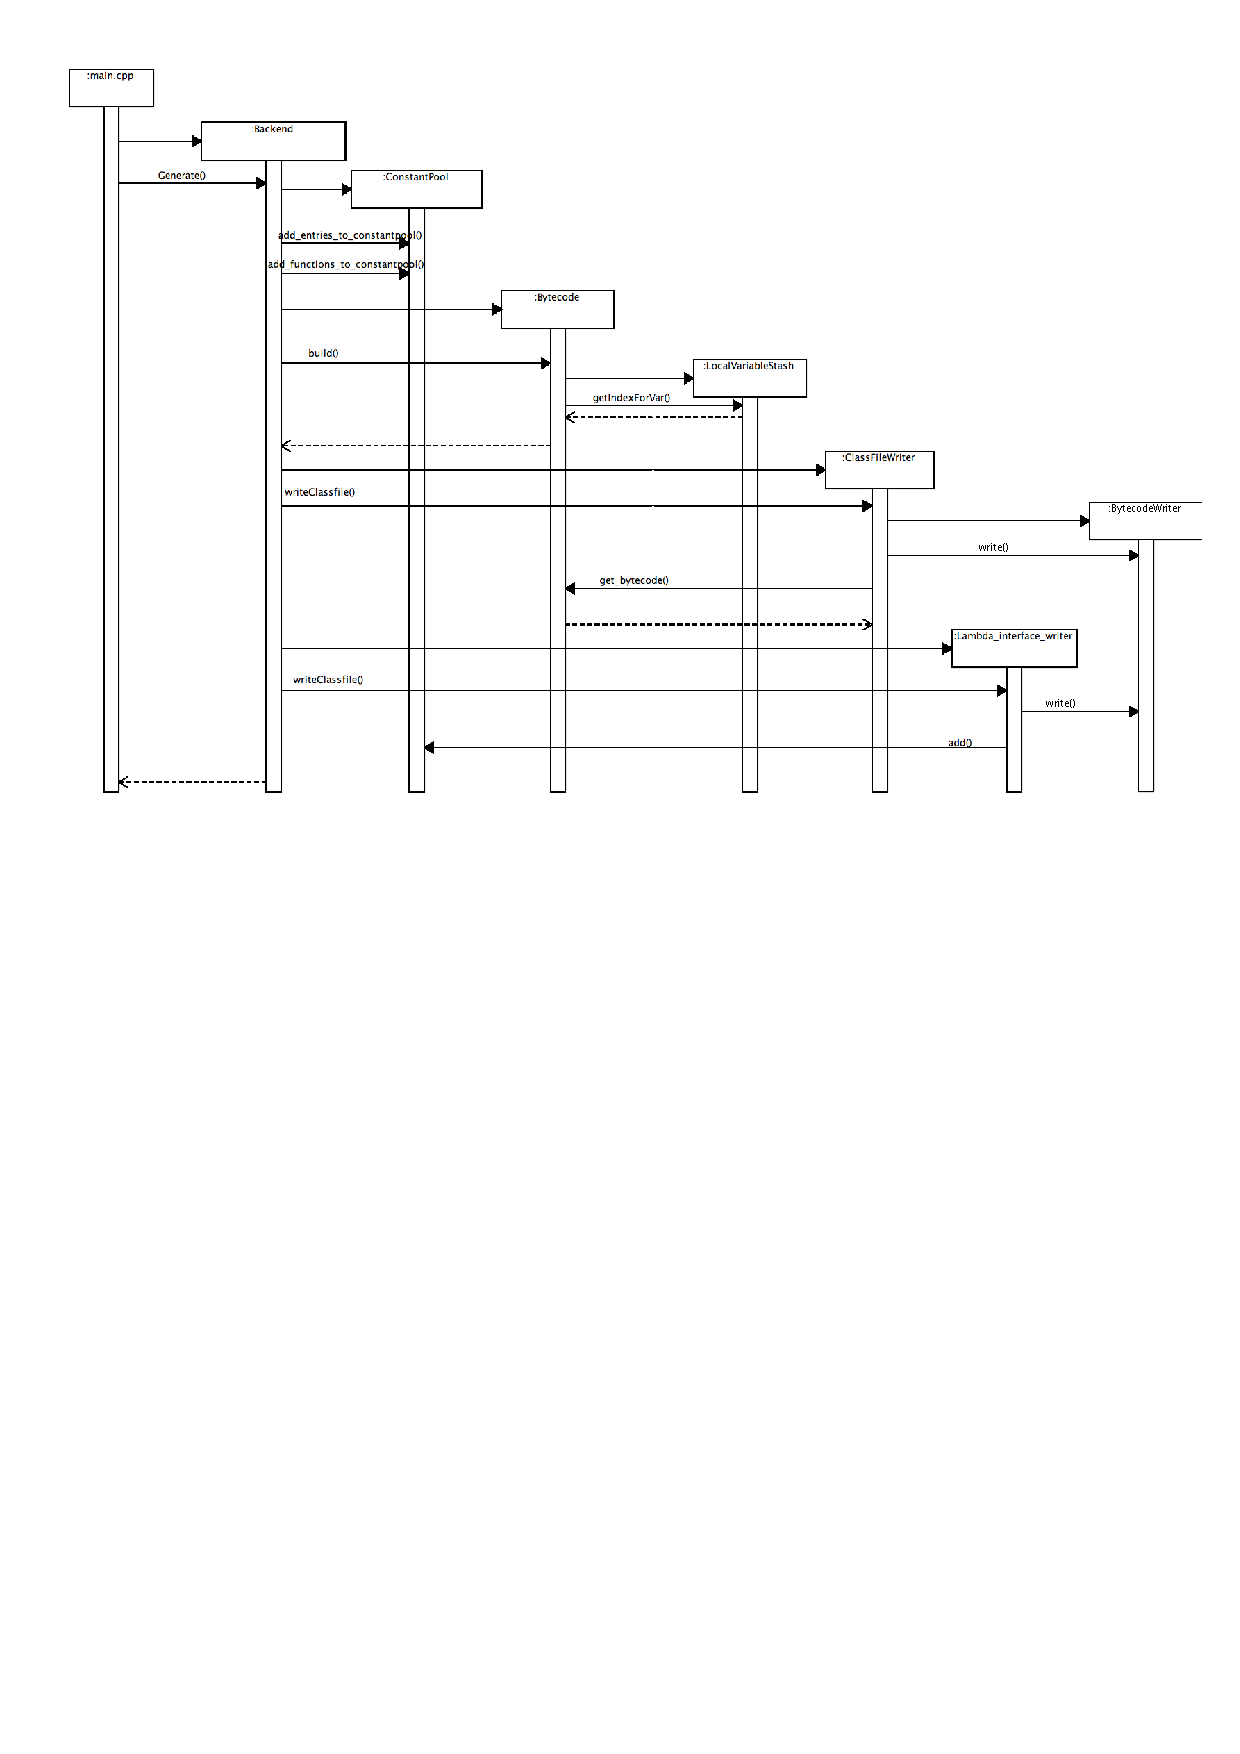
\includegraphics[width=\textwidth]{Sequenz}
\end{center}
\end{figure}
\end{frame}

\begin{frame}[fragile]{Backend Sequenzdiagramm Zweiter Teil}
\begin{figure}[htp]
\begin{center}
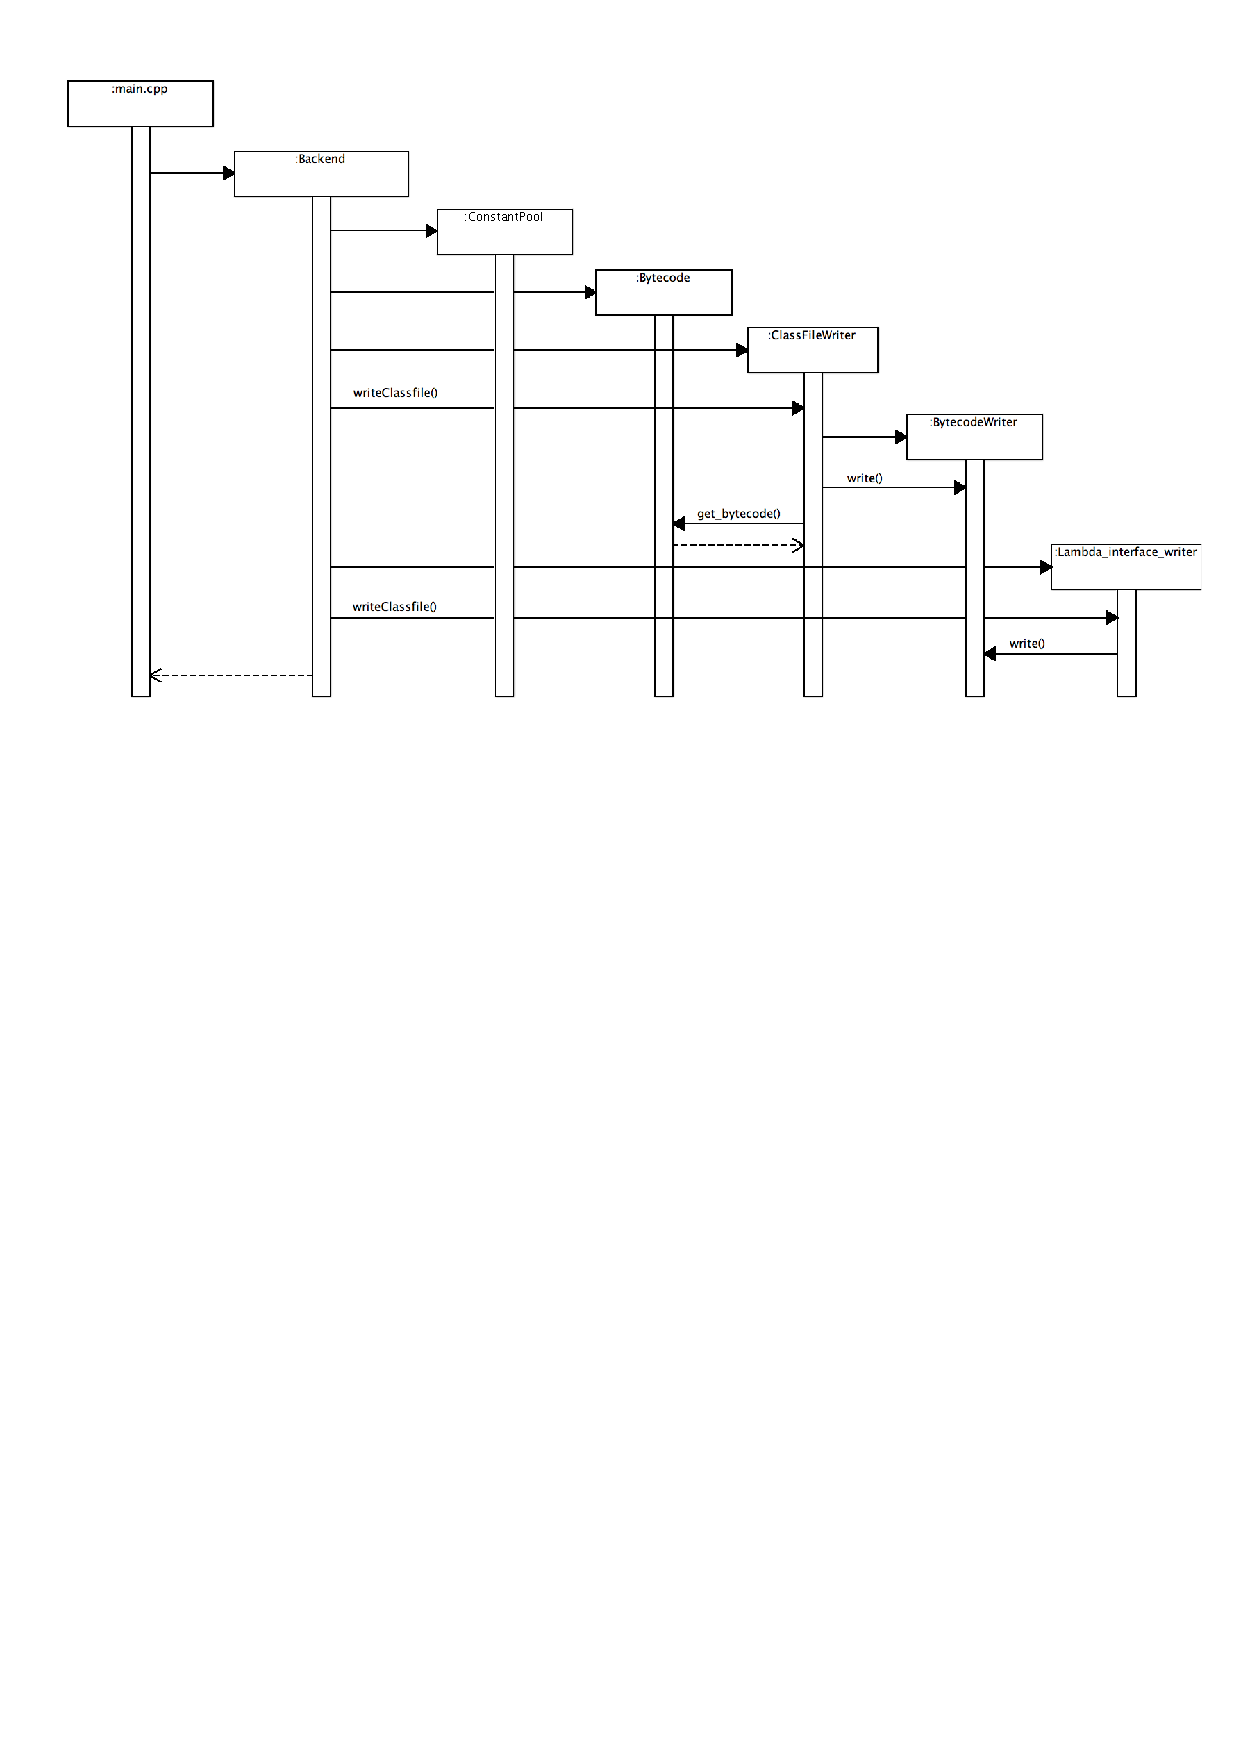
\includegraphics[width=\textwidth]{unten}
\end{center}
\end{figure}
\end{frame}


\begin{frame}[fragile]{Organisation und Probleme}

\pause
Organisation
\pause
  \begin{itemize}
  \item Hauptsächlich Teamspeak und Git Kommentarbereich
  \pause
  \item Außerdem XMPP und E-Mail 
  \pause
  \end{itemize}
Probleme
\pause
  \begin{itemize}
  \item Classfiles waren anfangs kompliziert zu durchblicken
  \pause
  \item Das Classfile-Gerüst war schwerer zu realisieren als die grundlegenden Funktionen
  \pause
  \item Einteilung der Meilensteine war für uns kontraproduktiv
  \end{itemize}
\end{frame}

\begin{frame}[fragile]{Beispiel}
Zum Abschluss:
  \begin{itemize}
  \item Eine von uns generierte Classfile
  \end{itemize}
\end{frame}
\subsection{Rail-Editor}

\begin{frame}{Rail-Editor}

\begin{figure}
  \begin{center}
    \leavevmode
      \includegraphics[width = .75\textwidth]{editor}
    \caption{Team Rail-Editor}
  \end{center}
\end{figure}

\end{frame}

\begin{frame}{Rail-Editor: Übersicht}

	Übersicht:
	\begin{itemize}
		\item Softwaretechnik
		\item Technische Aspekte
		\item Live-Demo
	\end{itemize}

\end{frame}

\pagebreak

\begin{frame}{Rail-Editor: Softwaretechnik}
	\begin{itemize}
		\item kleines Team $\rightarrow$ Kommunikation per Email
		\item direkte Reaktionen auf Emails (an alle geschickt)
		\item zuerst zwei, nach dem ersten Milestone drei Mitglieder
		\begin{itemize}
			\item bessere Arbeitsverteilung
		\end{itemize}
		\item Teilnahme an Daily Scrums (montags und mittwochs)
		\item zusätzliche Team-Meetings außer donnerstags
		\begin{itemize}
			\item produktives Arbeiten durch Pair-Programming
		\end{itemize}
		\item gute Kommunikation innerhalb des Teams
		\item anfangs spärliche Kommunikation mit anderen Teams
	\end{itemize}
\end{frame}

\begin{frame}{Rail-Editor: Technische Aspekte I}
	\begin{itemize}
		\item \textit{QT} für Programmierung der grafischen Benutzeroberfläche
		\item Signal- und Slottechnik
		\item Eventverarbeitung für Maus- und Tastendrücke
		\item Basisklassen abgeleitet und Funktionalitäten erweitert
		\item Graphstruktur für Syntax-Highlighting
		\begin{itemize}
			\item internes Backend
		\end{itemize}
		\item Smart-Cursor und Grab-Modus
		\begin{itemize}
			\item für intuitives Schreiben von Quellcode
			\item siehe Live-Demo
		\end{itemize}
	\end{itemize}
\end{frame}

\begin{frame}{Rail-Editor: Technische Aspekte II}
	\begin{itemize}
		\item Main-Window als \textit{Brain}
		\begin{itemize}
			\item Weiterleitung an Child-Widgets
		\end{itemize}
		\item Undo-Redo-Funktionalität
		\begin{itemize}
			\item abstrakte Klasse
			\item wird durch konkrete Aktionen implementiert
		\end{itemize}
		\item Compiler-Einbindung
		\begin{itemize}
			\item Funktionen: Build, Run, Stop
			\item auch der Rail-Interpreter kann verwendet werden
		\end{itemize}
		\item \textit{Preferences} (Editor-Einstellungen)
		\begin{itemize}
			\item persistent gespeichert
		\end{itemize}
	\end{itemize}

\end{frame}

\begin{frame}{Rail-Editor: Technische Aspekte III}
	\begin{figure}
		\centering
		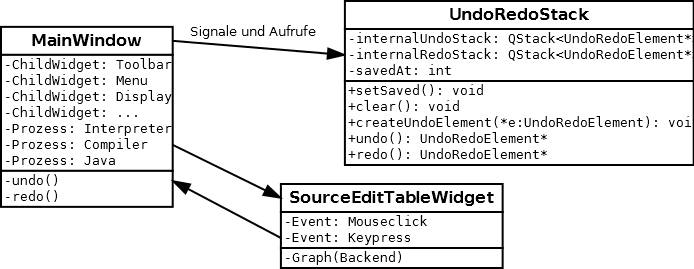
\includegraphics[width=0.7\textwidth]{editor-uebersicht}
	\end{figure}
\end{frame}

\subsection{Fazit}

\begin{frame}{Fazit}

	\pause
	Wir hatten
	\pause
	\begin{itemize}
		\item Ziemlich viel Arbeit
		\pause
		\item Einige Coding-Marathons
		\pause
		\item Mindestens 5 Nervenzusammenbr\"uche wegen des C++ 11 Standards
		\pause
		\item Mindestens 20 Nervenzusammenbr\"uche weil jemand auf die Idee gekommen ist Eclipse zu verwenden
		\pause
		\item Noch ein paar Nervenzusammenbr\"uche mehr wegen der Fehlermeldungen des GCC
		\pause
		\item \"Uber 20 Mal "Oh Nein, das Projekt kompiliert nicht mehr!"
		\pause
		\item Mindestens 4 Wochen lang eine kaputte .class-Datei generiert
		\pause
		\item Zahllose WTF-Momente
	\end{itemize}

\end{frame}

\begin{frame}{Fazit}

	\pause
	Außerdem haben wir:
	\pause
	\begin{itemize}
		\item Viel gelernt
		\pause
		\item Ziemlich viel Spaß gehabt
		\pause
		\item Super Teamgeist bewiesen
		\pause
		\item Regelm\"aßig Kekse gegessen
		\pause
		\item Also kurz: Spiel, Spaß und Schokolade
		\pause
	\end{itemize} \newline \newline \vspace{5mm}	\textbf{\textcolor{fu-green}{Also auch wenn wir das Projekt Jail++ getauft haben	kam uns das Projekt nicht wie ein Gef\"angnisaufenthalt vor.}}
	
	\begin{figure}
		  \begin{center}
		    \leavevmode
		      
\includegraphics[width = .2\textwidth]{smiley}
		  \end{center}
		\end{figure}
	
\end{frame}

\begin{frame}{Fazit}

	\begin{figure}
	  \begin{center}
	    \leavevmode
	      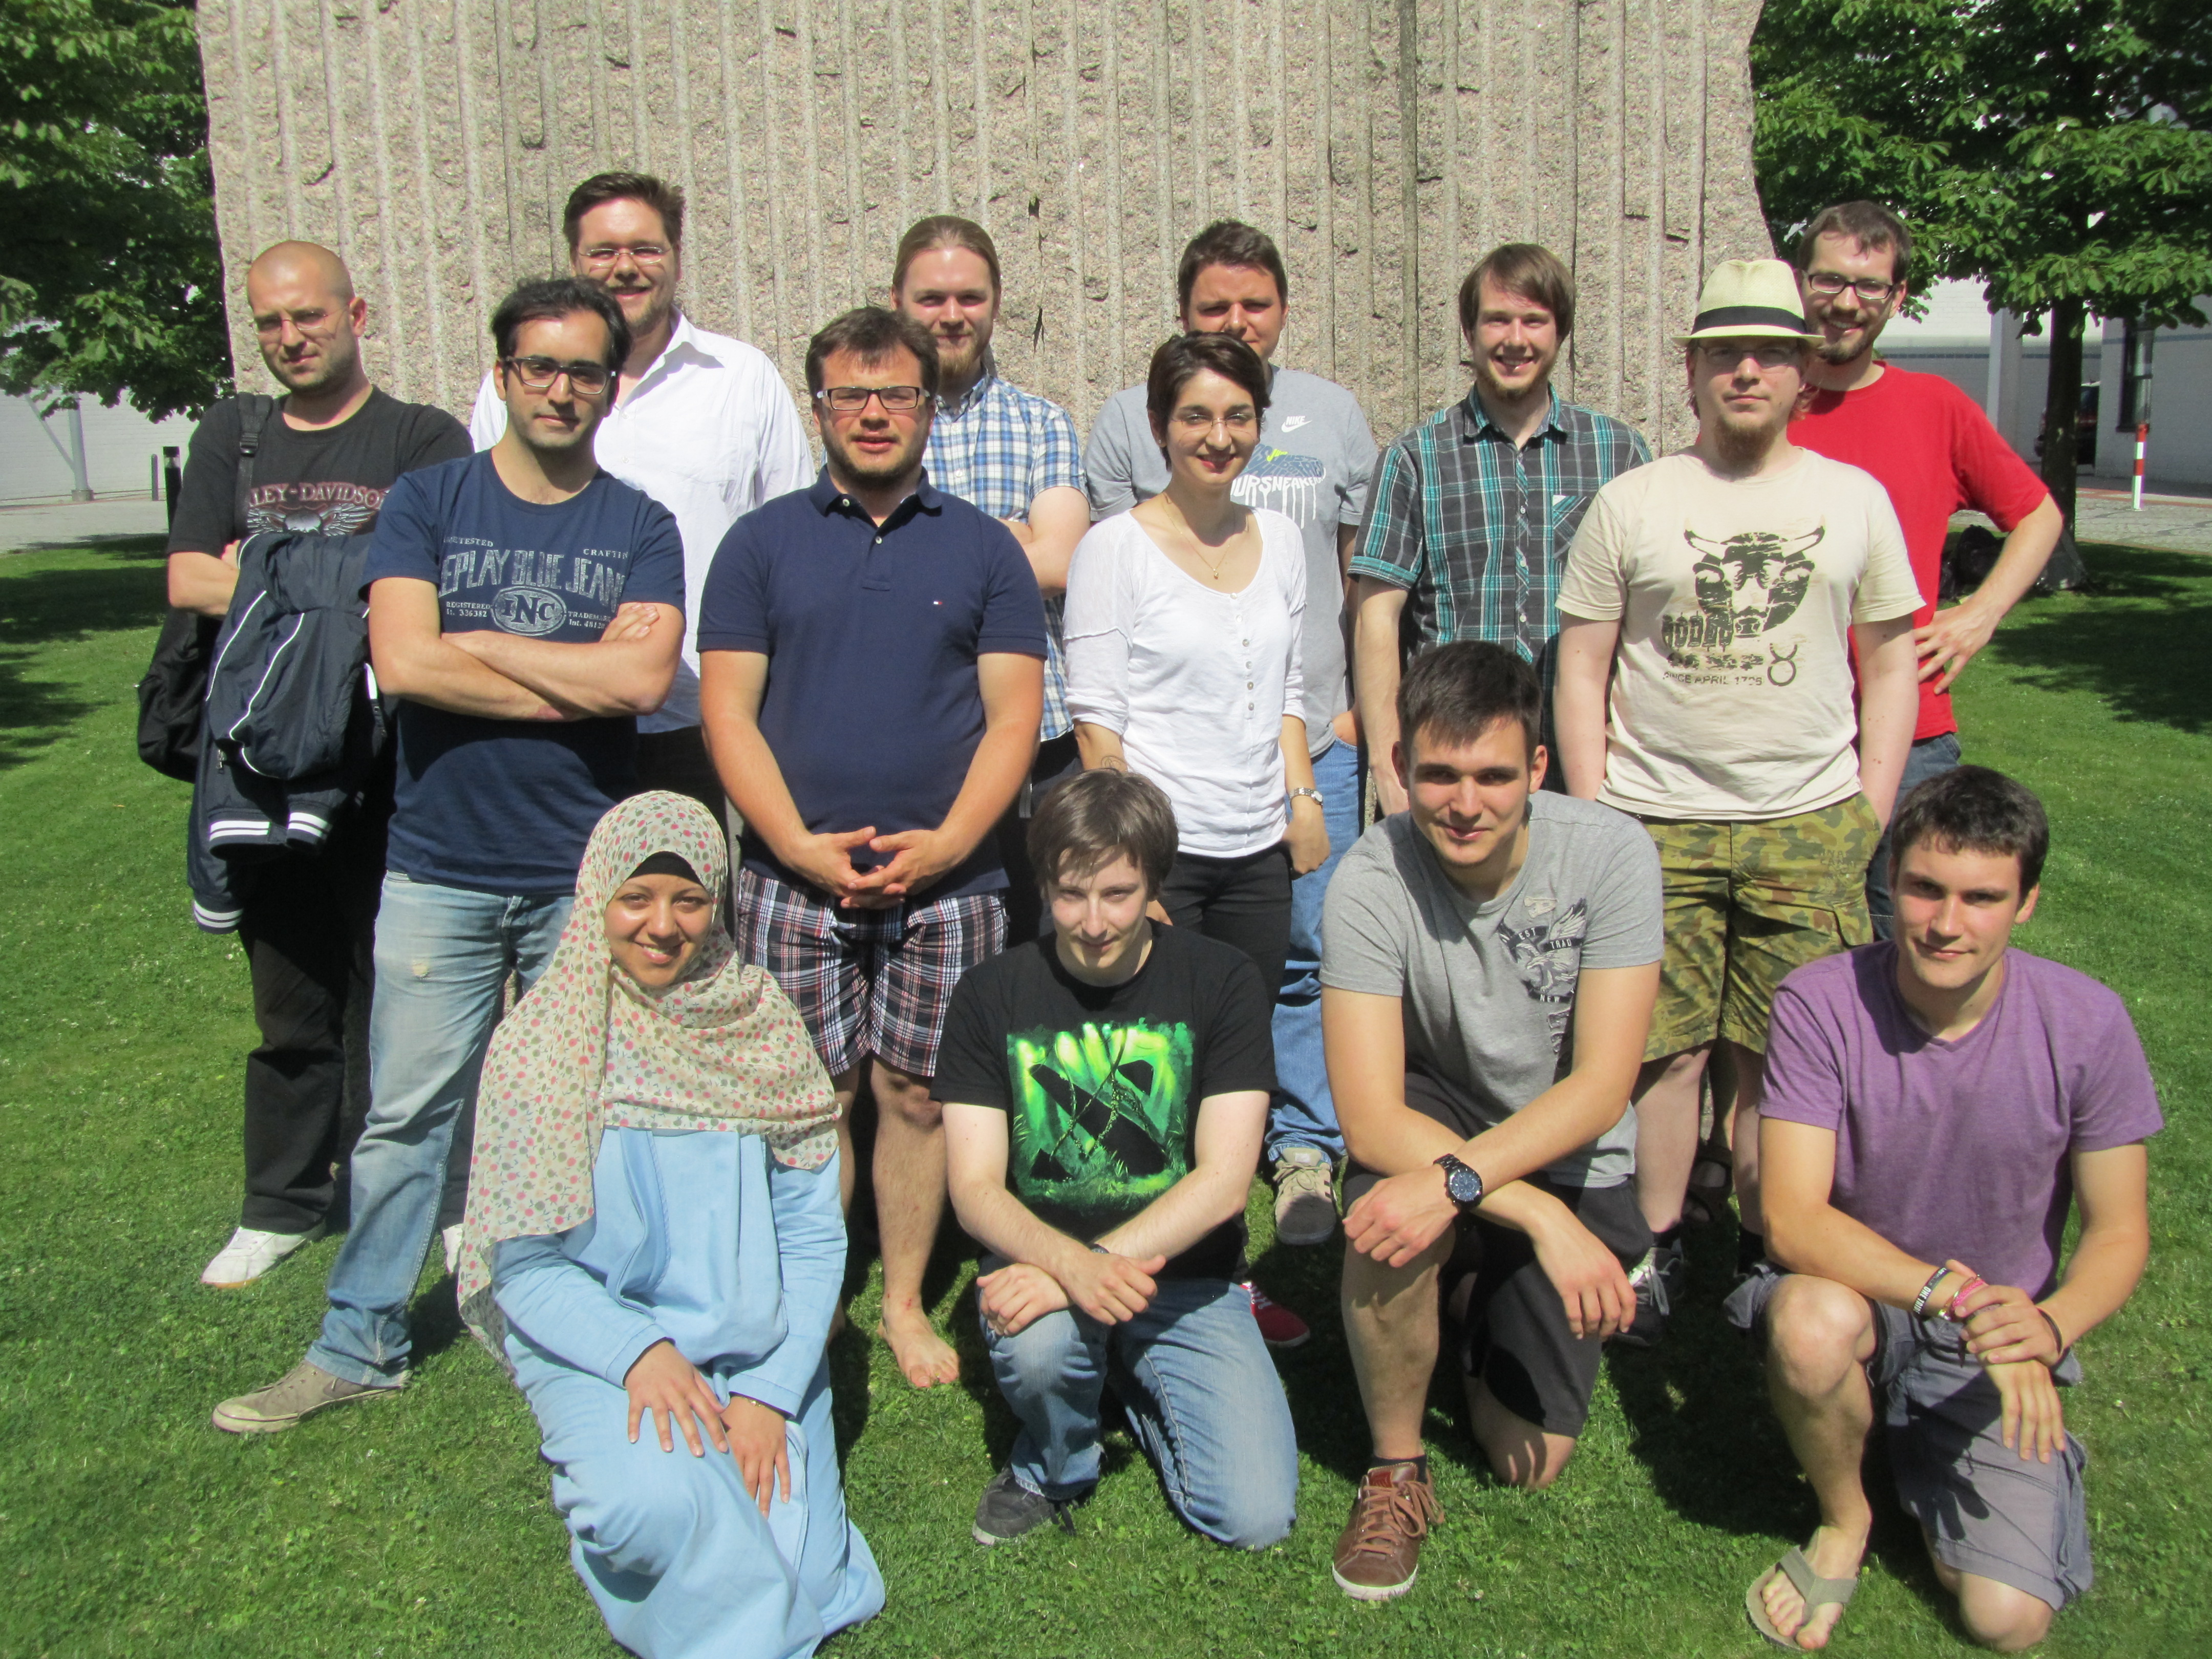
\includegraphics[width = .75\textwidth]{gruppe}
	    \caption{Jail Constructions Ltd. (auch bekannt als C++ Gruppe)}
	  \end{center}
	\end{figure}

\end{frame}



\end{document}
